\documentclass{beamer}

\usepackage[utf8]{inputenc}
\usecolortheme{beaver}
\usepackage{caption}
\usepackage{subcaption}
\usepackage{mathtools}
\usepackage{todonotes}
\usepackage{amsmath}
\usepackage{bm}
\usepackage{listings}
\usepackage{ragged2e}
\usepackage{titlecaps}
\usepackage{fancyvrb}

\def\ci{\perp\!\!\!\!\!\perp}

\newtheorem{proposition}{Proposition}
\Addlcwords{for a is but and with of in as the etc on to if}

\setbeamertemplate{section in toc}{\inserttocsectionnumber.~\inserttocsection}
\usetheme{Boadilla}
\makeatletter
\setbeamertemplate{footline}{%
    \leavevmode%
    \hbox{%
        \begin{beamercolorbox}[wd=.3\paperwidth,ht=2.25ex,dp=1ex,center]{author in head/foot}%
            \usebeamerfont{author in head/foot}\insertshortauthor\expandafter\beamer@ifempty\expandafter{\beamer@shortinstitute}{}{~~(\insertshortinstitute)}
        \end{beamercolorbox}%
        \begin{beamercolorbox}[wd=.55\paperwidth,ht=2.25ex,dp=1ex,center]{title in head/foot}%
            \usebeamerfont{title in head/foot}\insertshorttitle
        \end{beamercolorbox}%
        \begin{beamercolorbox}[wd=.15\paperwidth,ht=2.25ex,dp=1ex,right]{date in head/foot}%
            \usebeamerfont{date in head/foot}\insertshortdate{}\hspace*{2em} \insertframenumber{} / \inserttotalframenumber\hspace*{2ex} 
        \end{beamercolorbox}}%
        \vskip0pt%
    }
\makeatother

\begin{document}

\title[]{Meta-Dependence in Conditional Independence Testing}
\date{}

\begin{frame}
	\begin{figure}
		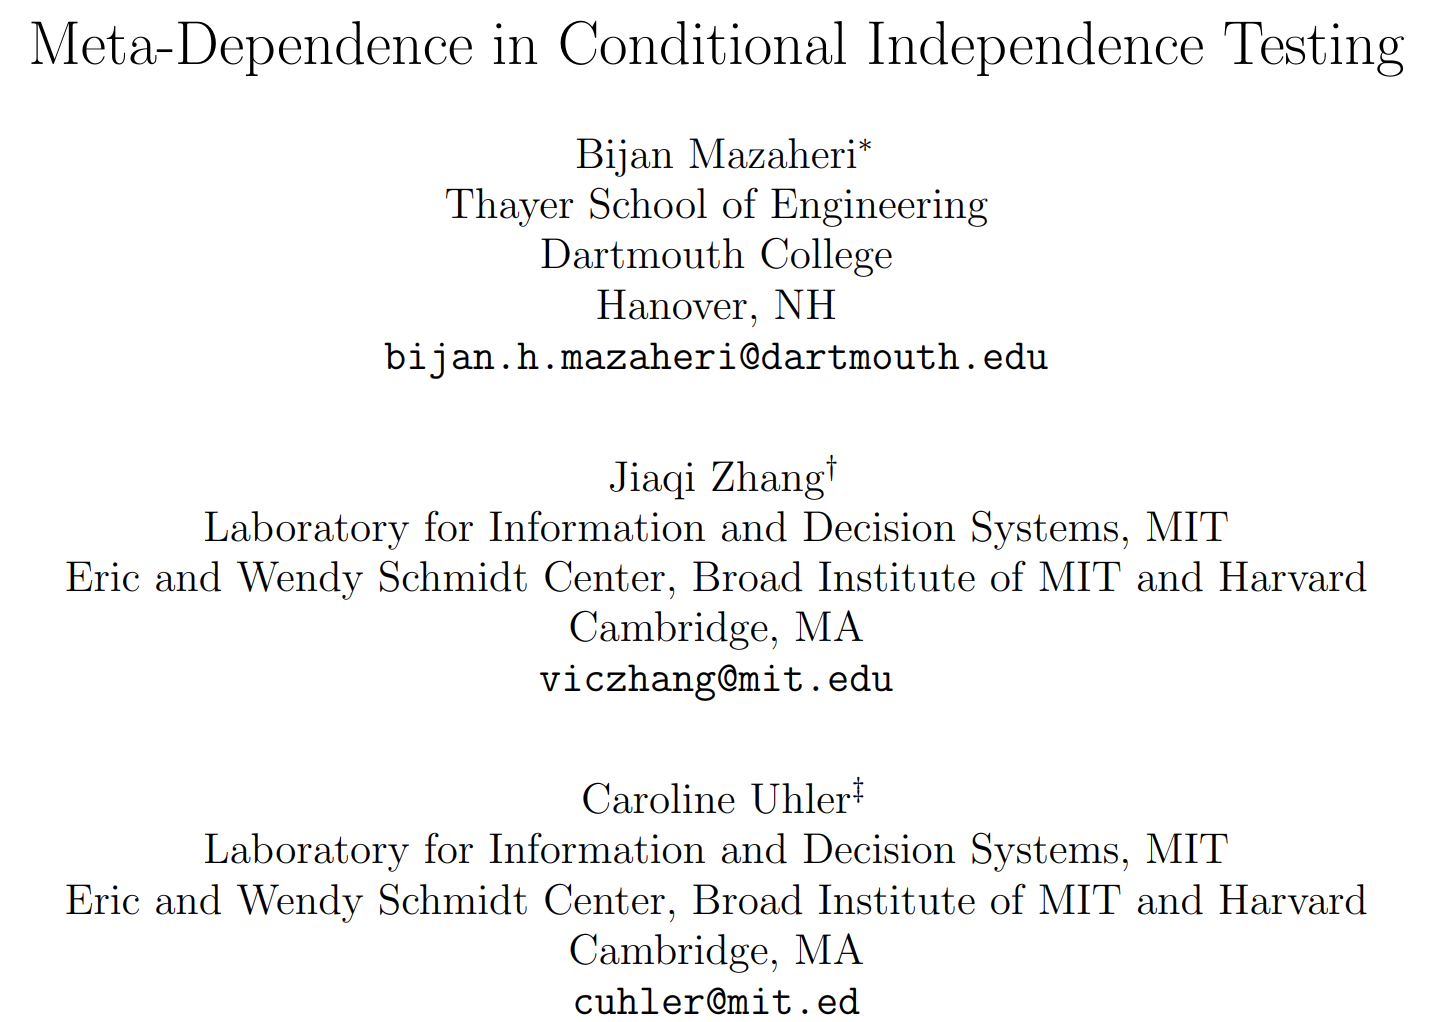
\includegraphics[scale=0.15]{imgs/title.png}
	\end{figure}
\end{frame}

\begin{frame}{Background}
\end{frame}

\begin{frame}{Problems with Causal Discovery}

\end{frame}

\begin{frame}{Proposed Solution Summary}
\end{frame}

\begin{frame}{Faithfulness}
\end{frame}

\begin{frame}{$\lambda$-strong Faithfulness}
	\begin{figure}
		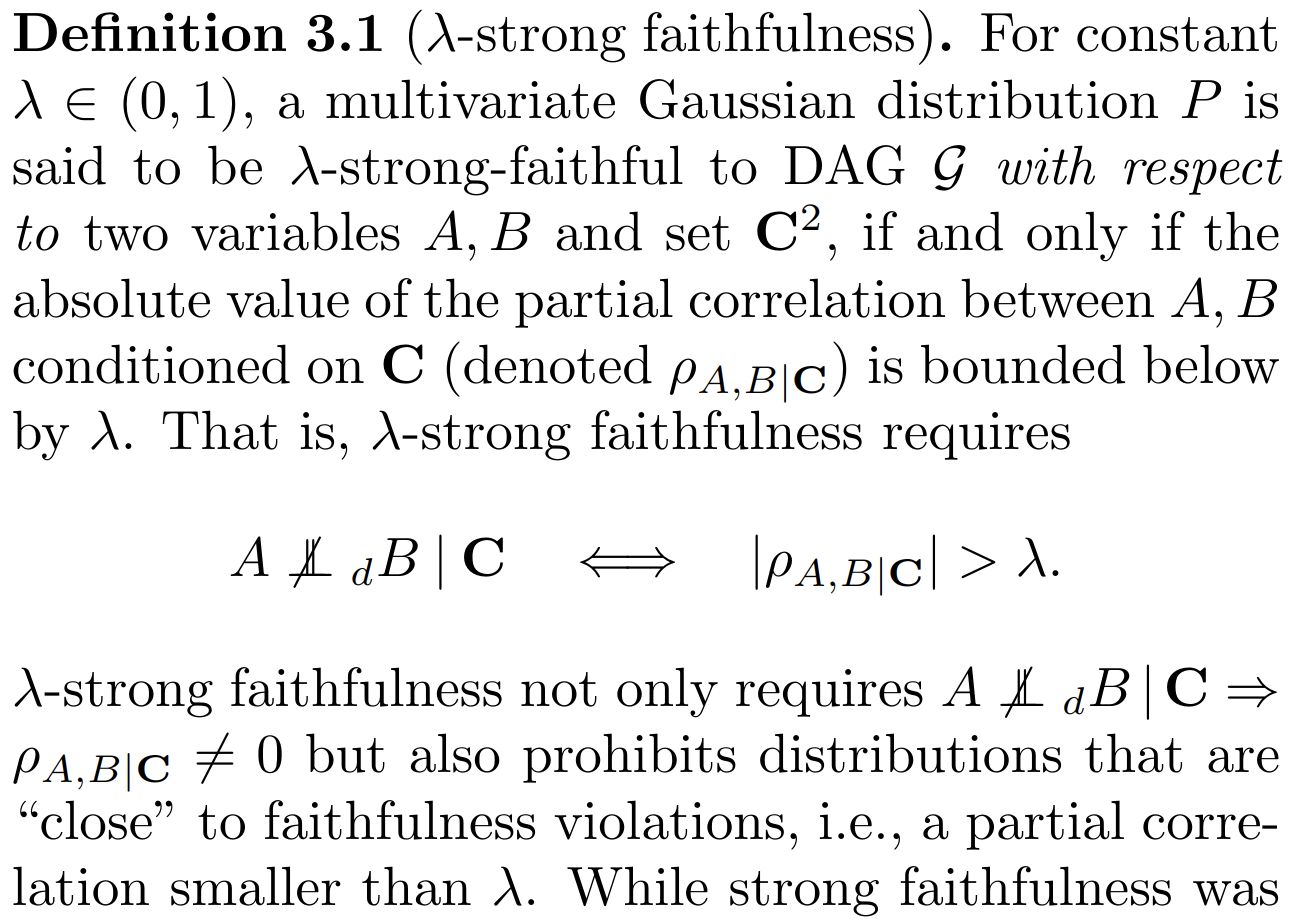
\includegraphics[scale=0.15]{imgs/def31.png}
	\end{figure}
\end{frame}

\begin{frame}{Dependence of Faithfulness}
	\begin{itemize}
		\item Examine the dependence between different faithfulness violations.
		\item Consider a joint distribution $ P $ generated from a DAG $ G $. 
		\item Local parameter perturbations on equation parameters to mimic estimator errors of empirical distributions on finite samples.
		\item Perturbations alter partial correlation between variables resulting in strong faithfulness violations.

	\end{itemize}
\end{frame}

\begin{frame}{Model Setup}
	\begin{itemize}
		\item Linear Additive Gaussian Model: Each variable $V = \sum_{U\in\text{pa}(V)} \theta_{UV}U + N_V$ where $N_V \sim \mathcal N(0,\sigma_V^2)$ and $N_V$’s are mutually independent.
	\end{itemize}
\end{frame}

\begin{frame}{Parameter Perturbations}
	\begin{itemize}
		\item Treat perturbations in the parameter space.
		\item Perturbations move the joint distribution through parameter space towards/away from CI manifolds.
		\item A single perturbation can approach multiple CI manifolds simultaneously.
	\end{itemize}
\end{frame}

\begin{frame}{Parameter Perturbations: Single Violation}
	$ A = N_A, \;\;\; B = \alpha A + N_B $
	\begin{itemize}
		\item Correlation: $ \rho_{AB} = \alpha $.
		\item For DAG $ A \rightarrow B $, the distribution is $ \alpha'$-strong faithful whenever $ \alpha > \alpha' $.
		\item Perturbation: Shift $ \alpha $ to $ \alpha' $ $ \implies $ violation of $ \alpha'$-strong faithfulness.
	\end{itemize}
\end{frame}

\begin{frame}{Parameter Perturbations: Multiple Violations}
	\begin{itemize}
		\item DAG: $ A \rightarrow B \rightarrow C, A \rightarrow C $.
		\item $ A = N_A, \;\;\; B = \alpha_1 A + N_B, \;\;\; C = \alpha_2 A + \beta B + N_C $.
		\item Correlations: $ \rho_{AB} = \alpha_1, \rho_{AC} = \alpha_2 + \alpha_1 \beta , \rho_{BC} = \alpha_1 \alpha_2 + \beta$.
		\item  Assuming DAG: $ A \rightarrow B \rightarrow C $, the distribution is faithful to G if $ A \not \ci B $ and $ A \not \ci C $ implying $ \rho_{AB} \ne 0 $ and $ \rho_{A,C} \ne 0 $.
	\end{itemize}	
\end{frame}

\begin{frame}{Parameter Perturbations: Multiple Violations}

\end{frame}


\begin{frame}{Empirical Results}
	\begin{figure}
		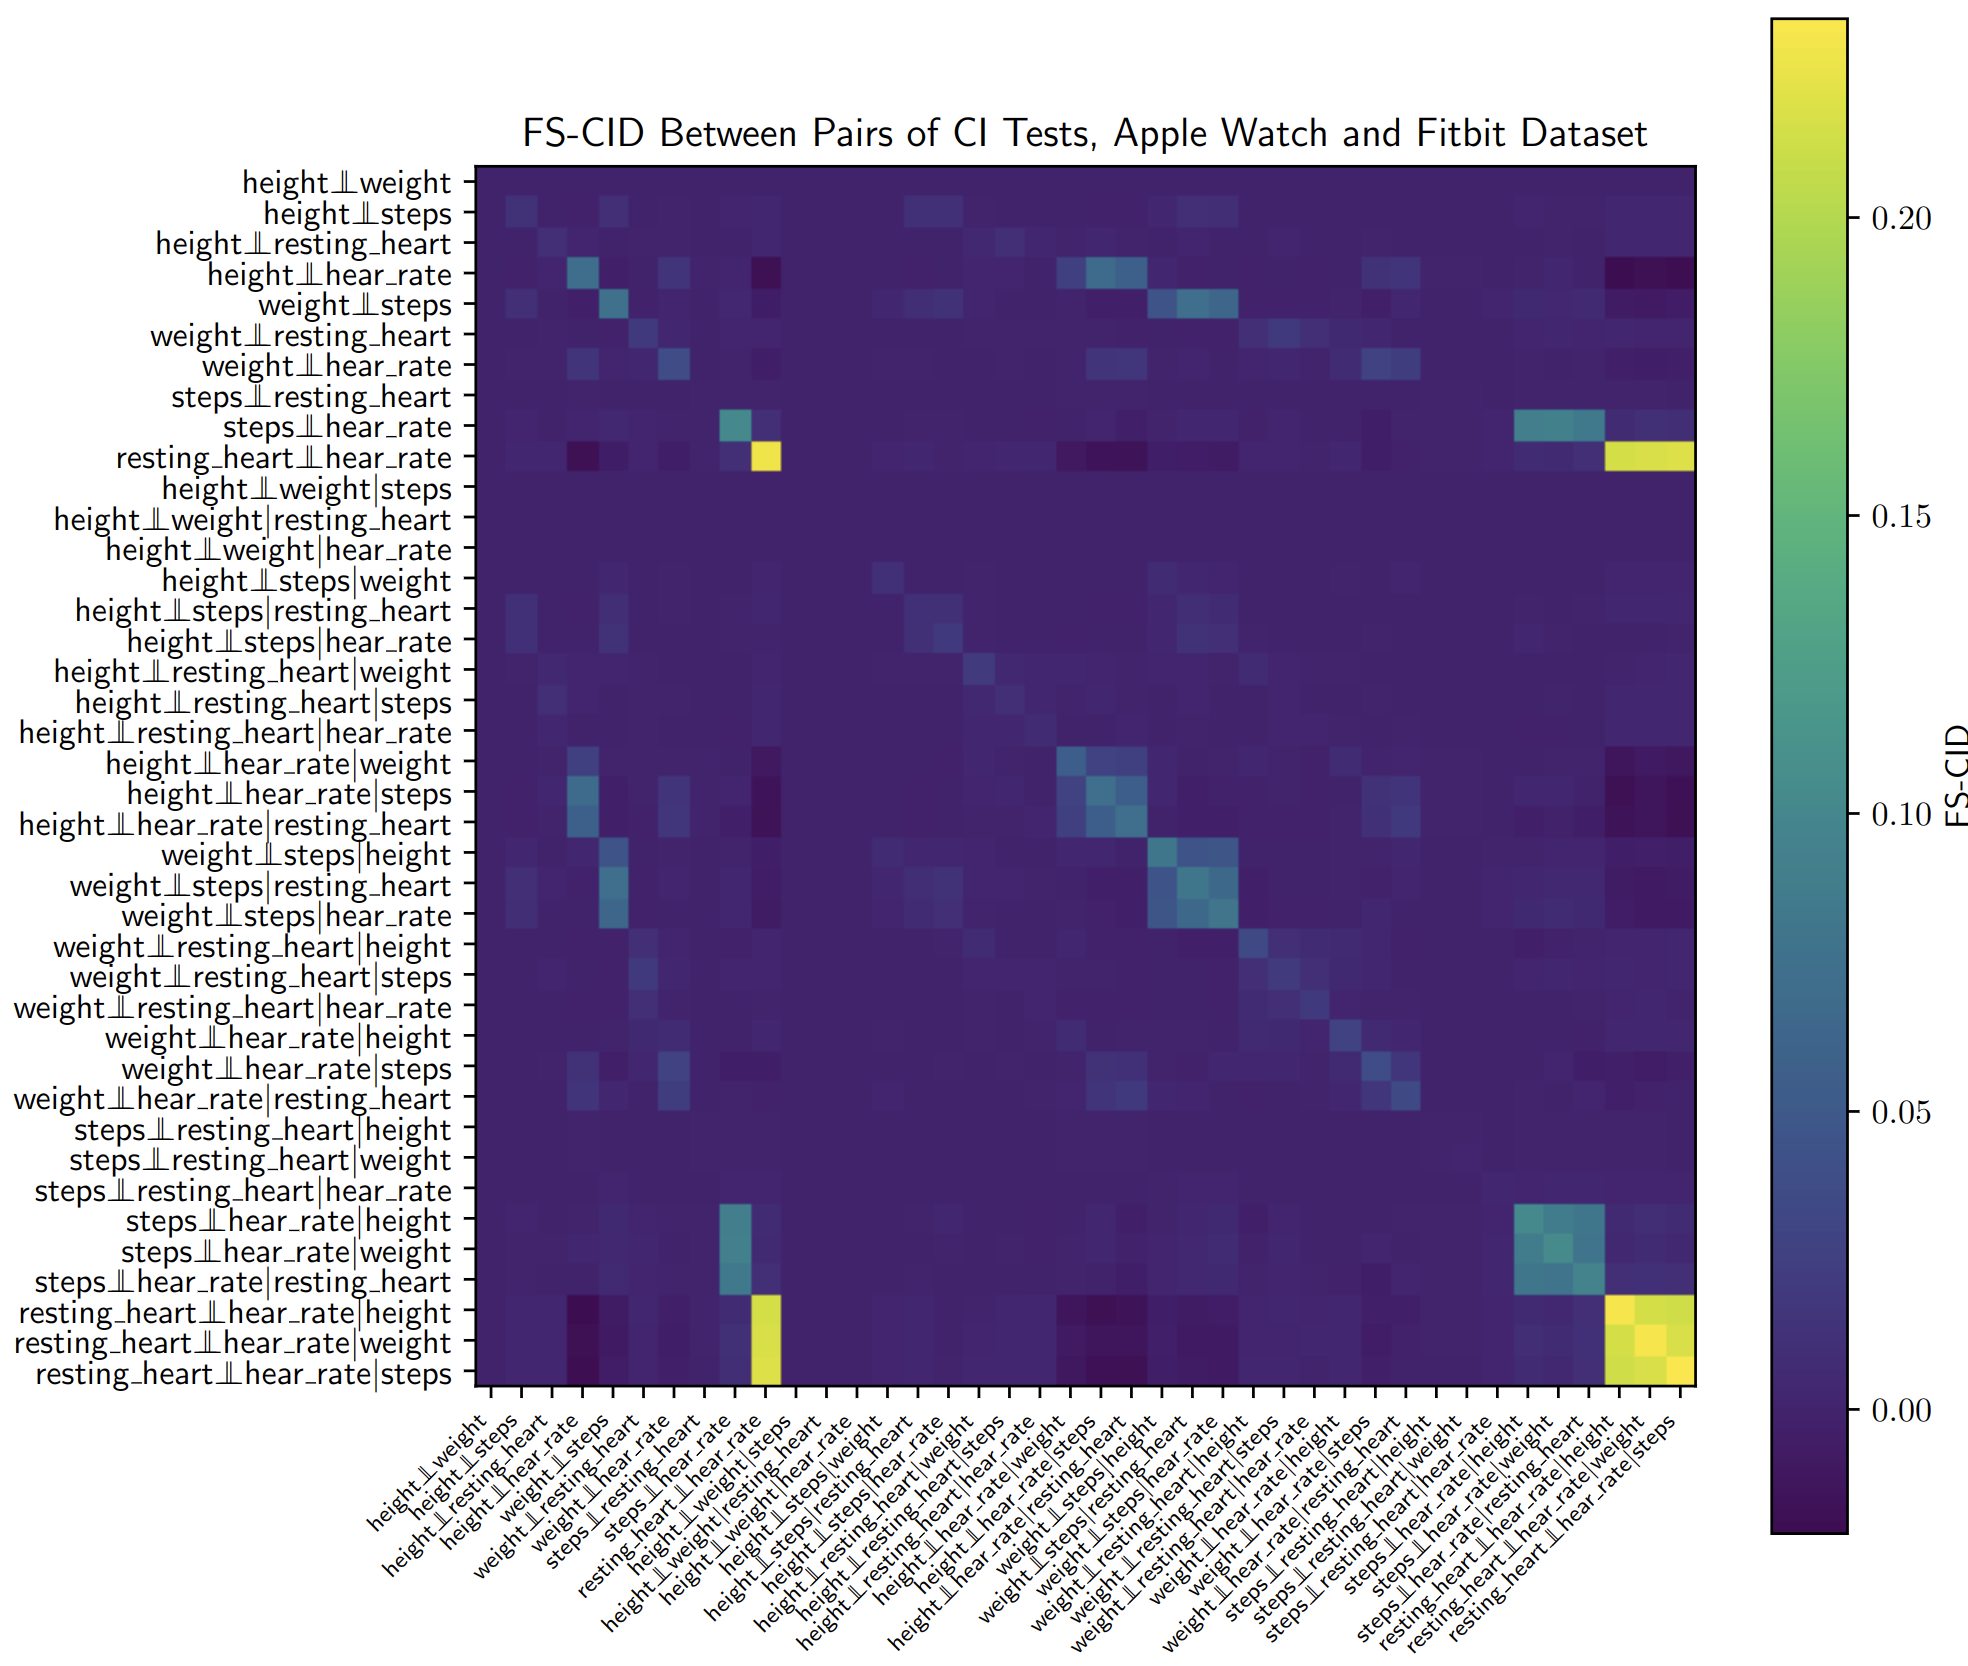
\includegraphics[scale=0.12]{imgs/empirical1.png}
	\end{figure}
\end{frame}

\begin{frame}{Empirical Results}
	\begin{figure}
		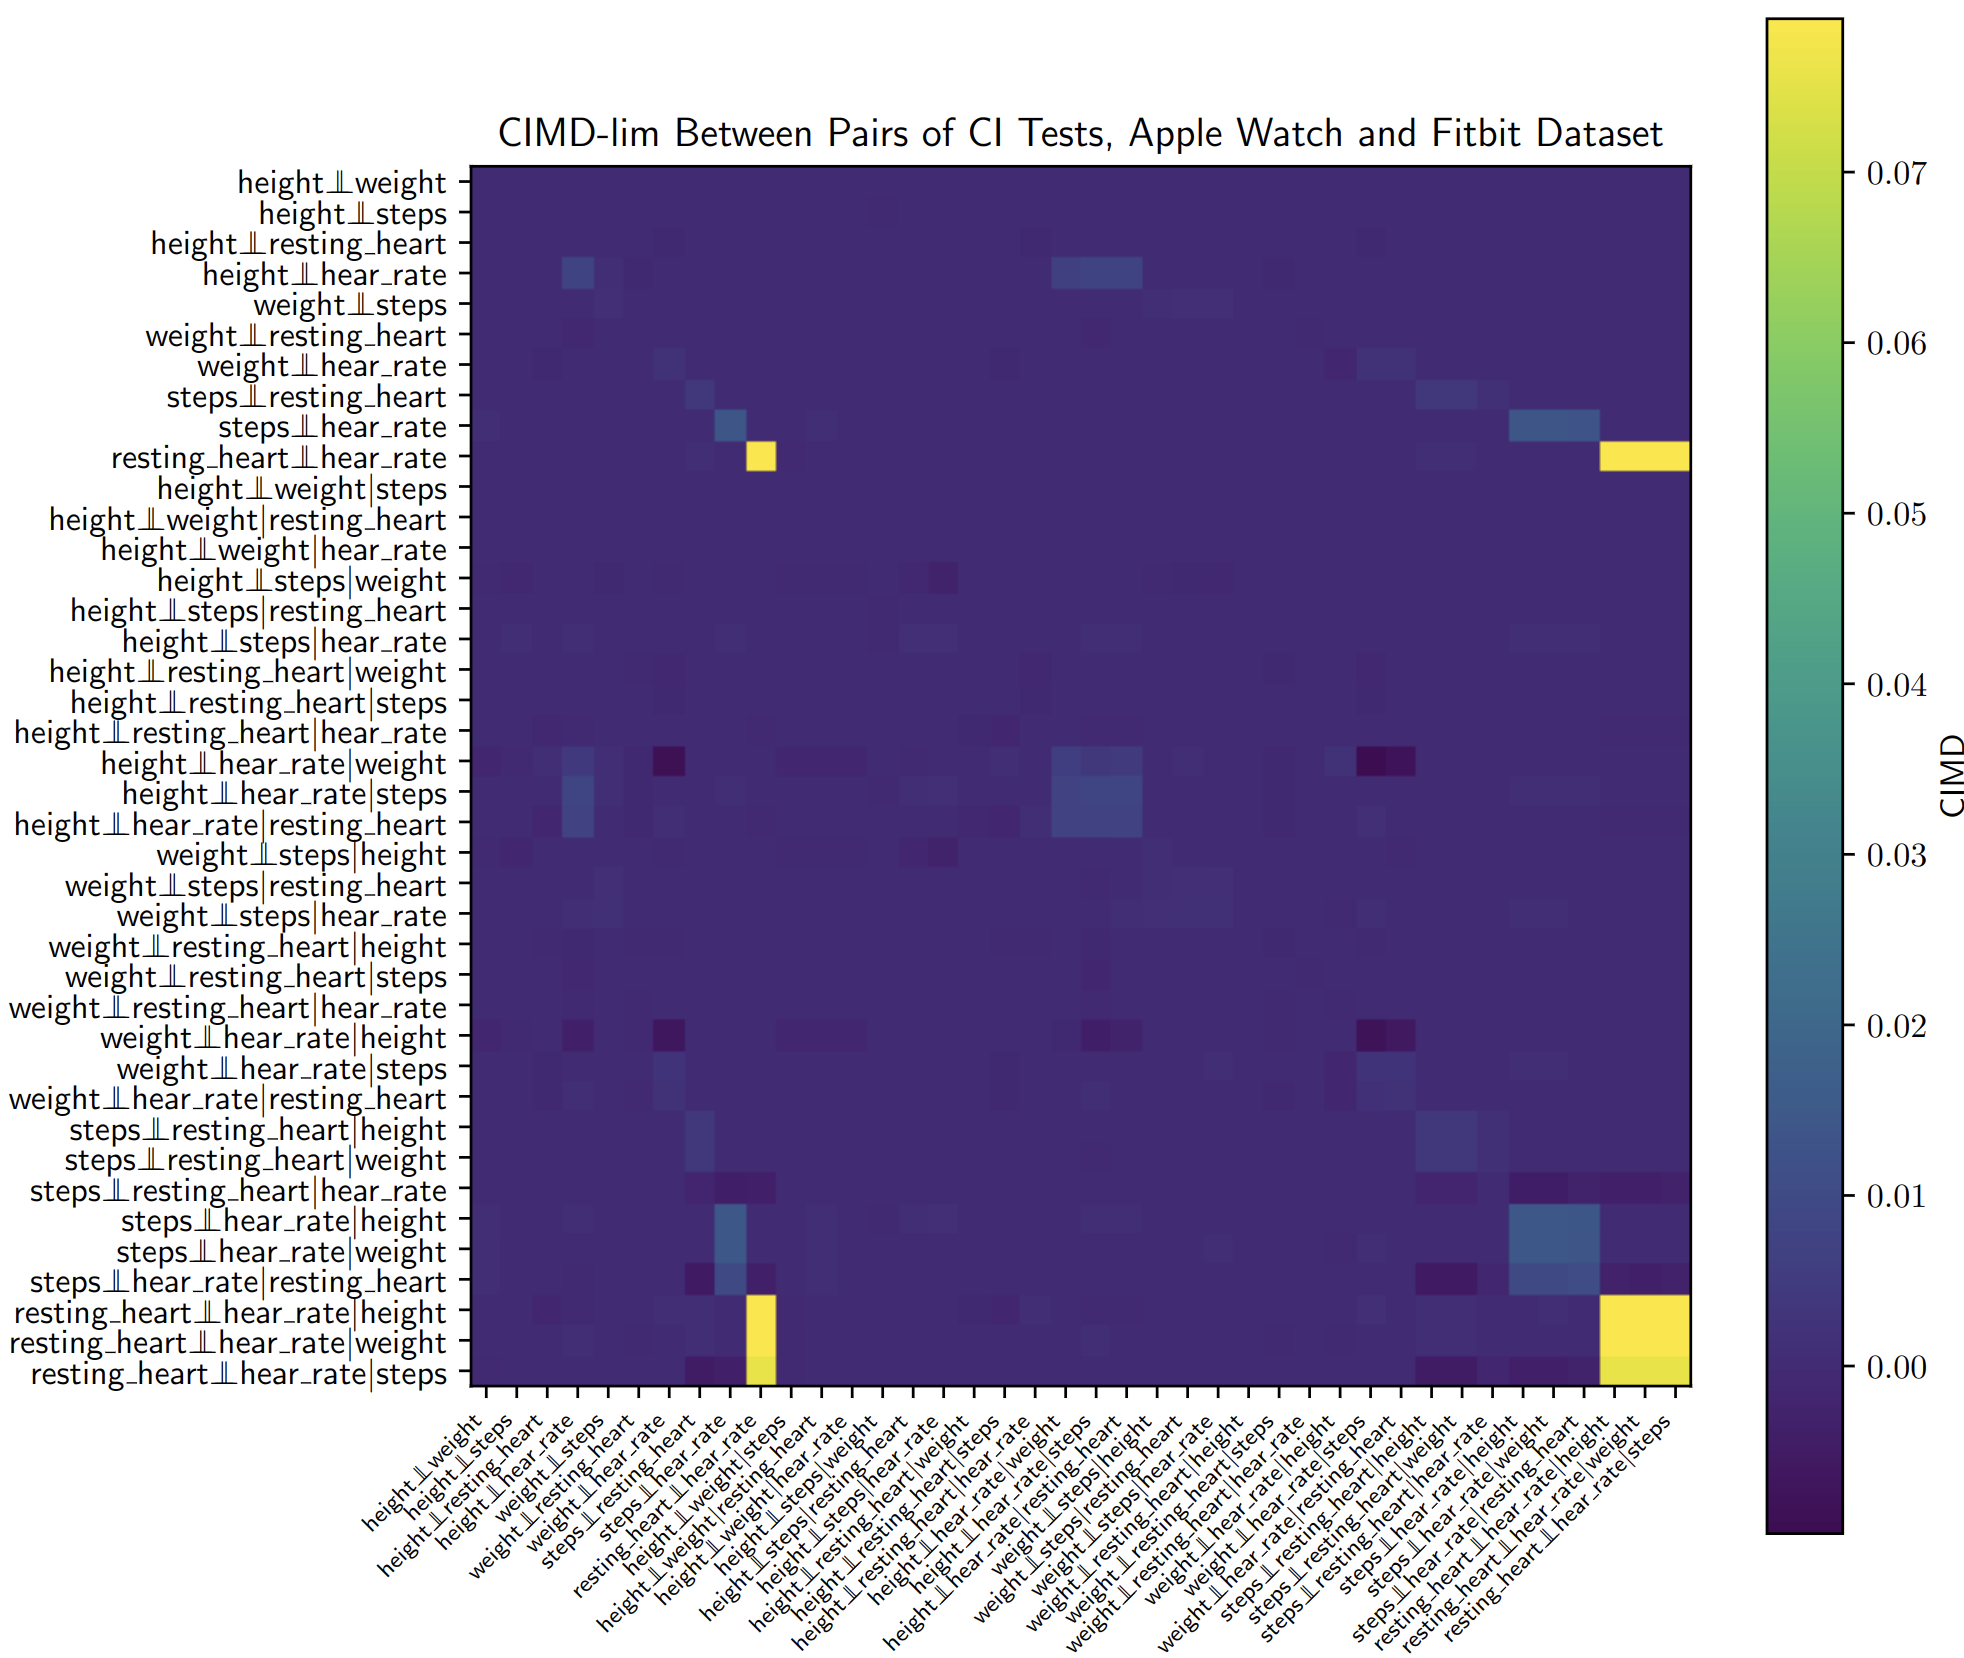
\includegraphics[scale=0.12]{imgs/empirical2.png}
	\end{figure}
\end{frame}

\end{document}
